\documentclass[12pt]{article}
\usepackage{amsmath}
\usepackage{tikz}
\usetikzlibrary{positioning}
\usepackage{graphicx}
\usepackage{times}         % Times New Roman
\usepackage{setspace}      % Para establecer el espaciado

\setstretch{1.0}           % Espaciado simpl

\title{La Sostenibilidad de la Deuda Técnica en una Empresa de Software}
\author{}
\date{}

\begin{document}

\maketitle

\tableofcontents % Genera el índice automáticamente
\newpage % Salto de página


\begin{abstract}
Este artículo explora la relación entre la deuda técnica en software y la sostenibilidad a largo plazo de una empresa de software. 
Utilizando conceptos de economía y derivadas, se muestra cómo la deuda técnica puede acumularse 
y afectar negativamente la productividad, la inversión y el crecimiento. 
Se presentan ecuaciones que modelan esta relación y se discute cómo mantener la sostenibilidad 
a través de un equilibrio adecuado entre la incurrencia y la reducción de la deuda técnica.
\end{abstract}

\section{Introducción}
La \textbf{deuda técnica} es un concepto en ingeniería de software que se refiere a los costos futuros incurridos por elegir una solución rápida y fácil en lugar de una solución mejor estructurada y de más alta calidad. A medida que una empresa de software continúa desarrollando y manteniendo su código base, la deuda técnica puede acumularse, lo que puede poner en riesgo la sostenibilidad a largo plazo de la empresa. Para analizar esta sostenibilidad, podemos utilizar conceptos de economía, particularmente los relacionados con la sostenibilidad de la deuda, como se describe en el libro \textit{Macroeconomía avanzada} de Argandoña, Gómez y Mochón.

\section{Definición y Acumulación de la Deuda Técnica}
La deuda técnica puede ser modelada de manera similar a la deuda financiera. Supongamos que \(D_t\) representa la cantidad de deuda técnica en el tiempo \(t\). La deuda técnica en un período \(t+1\) puede ser expresada como:

\[
D_{t+1} = D_t + N_t - R_t
\]

donde:
\begin{itemize}
    \item \(N_t\) es la nueva deuda técnica incurrida en el período \(t\),
    \item \(R_t\) es la reducción de la deuda técnica (refactorización, corrección de errores, etc.) en el período \(t\).
\end{itemize}

\section{Costo de la Deuda Técnica}
La deuda técnica tiene un costo asociado, que puede ser modelado como un interés sobre la deuda acumulada. Si \(i\) es la tasa de interés efectiva sobre la deuda técnica, el costo adicional en el tiempo \(t\) debido a la deuda acumulada es \(iD_t\). Por lo tanto, el costo total en el período \(t\) es:

\[
C_t = iD_t + R_t
\]

\section{Sostenibilidad de la Deuda Técnica}
Para evaluar la sostenibilidad de la deuda técnica, podemos adaptarnos al concepto de sostenibilidad de la deuda pública. Una deuda es sostenible si el crecimiento de la deuda no excede la capacidad de la empresa para gestionarla. Si consideramos que la empresa tiene un presupuesto de desarrollo \(B_t\) en cada período, la condición de sostenibilidad sería:

\[
iD_t + R_t \leq B_t
\]

Esto significa que la suma del costo del interés sobre la deuda técnica y la cantidad dedicada a reducirla debe ser menor o igual al presupuesto de desarrollo de la empresa.

\section{Deducción Lógica de la Insostenibilidad}
Si la empresa no puede reducir suficientemente la deuda técnica \(R_t\) o si el interés sobre la deuda técnica \(i\) es demasiado alto en comparación con el presupuesto \(B_t\), la deuda técnica crecerá sin control, poniendo en riesgo la operación de la empresa. Matemáticamente, si:

\[
iD_t + N_t > B_t
\]

entonces, la deuda técnica crecerá en cada período:

\[
D_{t+1} > D_t
\]

En el largo plazo, esta situación lleva a una espiral de deuda técnica que consume una parte cada vez mayor del presupuesto de la empresa, disminuyendo su capacidad para innovar y responder a nuevas demandas del mercado.

\section{Ejemplo Numérico}
Supongamos que una empresa tiene los siguientes parámetros:

\begin{itemize}
    \item Deuda técnica inicial: \(D_0 = 100\)
    \item Nueva deuda técnica por período: \(N_t = 20\)
    \item Reducción de la deuda técnica por período: \(R_t = 15\)
    \item Tasa de interés sobre la deuda técnica: \(i = 0.05\)
    \item Presupuesto de desarrollo por período: \(B_t = 50\)
\end{itemize}

Evaluamos la sostenibilidad:

Para \(t = 0\):

\[
C_0 = 0.05 \times 100 + 15 = 5 + 15 = 20 \leq 50
\]

Para \(t = 1\):

\[
D_1 = 100 + 20 - 15 = 105
\]
\[
C_1 = 0.05 \times 105 + 15 = 5.25 + 15 = 20.25 \leq 50
\]

Para \(t = 2\):

\[
D_2 = 105 + 20 - 15 = 110
\]
\[
C_2 = 0.05 \times 110 + 15 = 5.5 + 15 = 20.5 \leq 50
\]

Podemos observar que en los primeros períodos, la deuda técnica es manejable. Sin embargo, si el presupuesto no aumenta o si la tasa de interés incrementa, eventualmente la deuda técnica podría superar el presupuesto disponible, haciendo la situación insostenible.

\section{Productividad y Deuda Técnica}
Para evaluar la sostenibilidad de la deuda técnica, debemos considerar la productividad de la empresa. Supongamos que \(P_t\) representa la productividad de la empresa en el tiempo \(t\). La productividad puede ser afectada negativamente por la deuda técnica, ya que un código base con alta deuda técnica puede ser más difícil de mantener y desarrollar. Podemos modelar esta relación como:

\[
P_t = P_0 - \alpha D_t
\]

donde:
\begin{itemize}
    \item \(P_0\) es la productividad inicial de la empresa,
    \item \(\alpha\) es un coeficiente que mide el impacto negativo de la deuda técnica sobre la productividad.
\end{itemize}

Para analizar cómo cambia la sostenibilidad de la deuda técnica en el tiempo, podemos tomar la derivada de \(D_t\) con respecto al tiempo:

\[
\frac{dD_t}{dt} = N_t - R_t
\]

Considerando la relación entre productividad y deuda técnica, podemos tomar la derivada de \(P_t\) con respecto al tiempo:

\[
\frac{dP_t}{dt} = -\alpha \frac{dD_t}{dt} = -\alpha (N_t - R_t)
\]

Esto muestra que la tasa de cambio en la productividad es proporcional a la tasa de cambio en la deuda técnica. Si la empresa no puede reducir suficientemente la deuda técnica \(R_t\) o si la nueva deuda técnica \(N_t\) es demasiado alta, la productividad disminuirá con el tiempo, poniendo en riesgo la sostenibilidad.


\section{Impacto de la Deuda Técnica en el Crecimiento de la Empresa}

La deuda técnica no solo afecta la productividad, sino que también puede tener un impacto significativo en el crecimiento general de una empresa de software. El crecimiento empresarial se puede modelar en términos de la capacidad de la empresa para aumentar su participación en el mercado, lanzar nuevos productos y mejorar la eficiencia operativa. Sin embargo, a medida que la deuda técnica se acumula, estas capacidades pueden verse comprometidas.

\subsection{Crecimiento Reducido debido a la Deuda Técnica}

El crecimiento de una empresa \(G_t\) en el tiempo \(t\) puede ser considerado como una función de la productividad \(P_t\) y la inversión en innovación \(I_t\):

\[
G_t = \beta P_t + \gamma I_t
\]

donde:
\begin{itemize}
    \item \( \beta \) es el coeficiente que mide la influencia de la productividad en el crecimiento.
    \item \( \gamma \) es el coeficiente que mide la influencia de la inversión en innovación en el crecimiento.
\end{itemize}

Dado que la deuda técnica \(D_t\) reduce la productividad, la tasa de crecimiento también disminuirá si la deuda técnica no se maneja adecuadamente:

\[
G_t = \beta (P_0 - \alpha D_t) + \gamma I_t
\]

Esto muestra que un aumento en la deuda técnica \(D_t\) reduce la tasa de crecimiento \(G_t\), a menos que la empresa aumente significativamente su inversión en innovación \(I_t\) para compensar la caída en la productividad.

\subsection{Efecto en la Innovación y Expansión}

Además, una alta deuda técnica puede desviar recursos financieros y humanos que de otro modo se habrían utilizado para la innovación y la expansión del negocio. La inversión en innovación \(I_t\) puede verse limitada por los costos crecientes de mantener y mejorar un código base con alta deuda técnica. En términos de presupuesto, si una mayor proporción \(C_t\) se dedica a la gestión de la deuda técnica, menos recursos estarán disponibles para invertir en crecimiento:

\[
B_t = C_t + I_t
\]

\[
I_t = B_t - C_t
\]

Si el costo de la deuda técnica \(C_t\) aumenta, la inversión en innovación \(I_t\) disminuye, lo que a su vez reduce el crecimiento \(G_t\) de la empresa:

\[
G_t = \beta (P_0 - \alpha D_t) + \gamma (B_t - C_t)
\]

En el largo plazo, esto puede llevar a una disminución de la competitividad en el mercado, limitando la capacidad de la empresa para crecer y sostenerse en un entorno dinámico.

\subsection{Ciclo Vicioso de Deuda Técnica}

Finalmente, si la deuda técnica no se gestiona adecuadamente, puede llevar a un ciclo vicioso donde la baja productividad reduce el crecimiento, y el crecimiento reducido limita la capacidad de la empresa para invertir en la reducción de la deuda técnica y la innovación. Este ciclo puede ser difícil de romper, especialmente si la deuda técnica alcanza niveles críticos.

Este ciclo vicioso se puede representar de la siguiente manera:

\begin{center}
    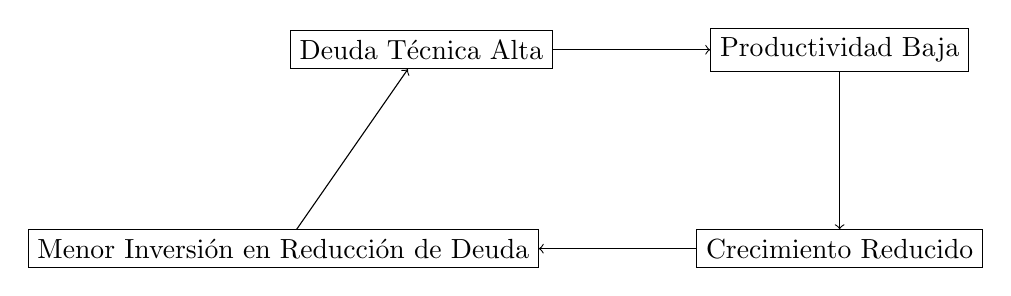
\begin{tikzpicture}[node distance=2cm, auto]
        % Nodes
        \node (a) [draw, rectangle] {Deuda Técnica Alta};
        \node (b) [draw, rectangle, right=of a] {Productividad Baja};
        \node (c) [draw, rectangle, below=of b] {Crecimiento Reducido};
        \node (d) [draw, rectangle, left=of c] {Menor Inversión en Reducción de Deuda};
    
        % Arrows
        \draw[->] (a) -- (b);
        \draw[->] (b) -- (c);
        \draw[->] (c) -- (d);
        \draw[->] (d) -- (a);
    \end{tikzpicture}
\end{center}

Por lo tanto, la gestión proactiva de la deuda técnica es crucial para mantener un crecimiento saludable y sostenido a lo largo del tiempo.


\section{Conclusión}

La deuda técnica, si no se maneja adecuadamente, puede poner en riesgo la sostenibilidad a largo plazo de una empresa de software. 
Usando conceptos de sostenibilidad de la deuda pública y la relación entre productividad e interés sobre la deuda técnica, se puede modelar y prever 
cómo la deuda técnica puede crecer hasta un punto en que los costos asociados superen la capacidad de la empresa para gestionarlos. 
La clave para la sostenibilidad es un equilibrio adecuado entre la incurrencia de nueva deuda técnica y su reducción sistemática, manteniendo una productividad 
que soporte los costos de la deuda técnica dentro de los límites del presupuesto disponible.

\section{Referencias}
\begin{itemize}
    \item Argandoña, A., Gómez, C., \& Mochón, F. (2006). \textit{Macroeconomía avanzada}. McGraw-Hill.
\end{itemize}

\end{document}
